\uuid{AGbd}
\exo7id{5545}
\titre{exo7 5545}
\auteur{rouget}
\organisation{exo7}
\datecreate{2010-07-15}
\isIndication{false}
\isCorrection{true}
\chapitre{Conique}
\sousChapitre{Parabole}
\module{Géométrie}
\niveau{L2}
\difficulte{}

\contenu{
\texte{
Déterminer l'orthoptique d'une parabole , c'est-à-dire l'ensemble des points du plan par
lesquels il passe deux tangentes à la parabole, perpendiculaires l'une à l'autre.
}
\reponse{
Dans un certain repère orthonormé, la parabole $\mathcal{P}$ admet une 
équation cartésienne de la forme $x^2=2py$. D'après la règle de dédoublement des termes, une équation de la tangente $\mathcal{T}_{x_0}$ en un point $(x_0,y_0)=\left(x_0,\frac{x_0^2}{2p}\right)$ de $\mathcal{P}$ est

\begin{center}
$xx_0=p(y+y_0)$.
\end{center}
Les tangentes en $M_0(x_0,y_0)$ et $M_1(x_1,y_1)$ sont perpendiculaires si et seulement si $x_0x_1+p^2=0$. L'orthoptique $\mathcal{C}$ est donc l'ensemble des points d'intersection de $\mathcal{T}_{x_0}$ et $\mathcal{T}_{-p^2/x_0}$ où $x_0$ décrit $\Rr^*$.
\begin{align*}\ensuremath
M(x,y)\in\mathcal{C}&\Leftrightarrow\exists x_0\in\Rr^*/\;\left\{
\begin{array}{l}
xx_0=p\left(y+\frac{x_0^2}{2p}\right)\\
-x\frac{p^2}{x_0}=p\left(y+\frac{p^3}{2x_0^2}\right)
\end{array}
\right.\Leftrightarrow\exists t\in\Rr^*/\;\left\{
\begin{array}{l}
tx-py=\frac{t^2}{2}\\
px+ty=-\frac{p^3}{2t}
\end{array}
\right.
\\
 &\Leftrightarrow\exists t\in\Rr^*/\;\left\{
\begin{array}{l}
x=\frac{1}{t^2+p^2}\left(\frac{t^3}{2}-\frac{p^4}{2t}\right)\\
y=\frac{1}{t^2+p^2}\left(-\frac{p^3}{2}-\frac{pt^2}{2}\right)
\end{array}
\right.\Leftrightarrow\exists t\in\Rr^*/\;\left\{
\begin{array}{l}
x=\frac{t^2-p^2}{2t}\\
\rule{0mm}{6mm}y=-\frac{p}{2}
\end{array}
\right..
\end{align*}
Maintenant, $\lim_{t\rightarrow 0^+}\frac{t^2-p^2}{2t}=-\infty$ et $\lim_{t\rightarrow +\infty}\frac{t^2-p^2}{2t}=+\infty$. Comme la fonction $t\mapsto\frac{t^2-p^2}{2t}$ est continue sur $]0,+\infty[$, quand $t$ décrit $]0,+\infty[$, $x=\frac{t^2-p^2}{2t}$ décrit $\Rr$. Finalement, l'orthoptique $\mathcal{C}$ est la droite d'équation $y=-\frac{p}{2}$ ou encore

\begin{center}
\shadowbox{
l'orthoptique d'une parabole est sa directrice.
}
\end{center}

$$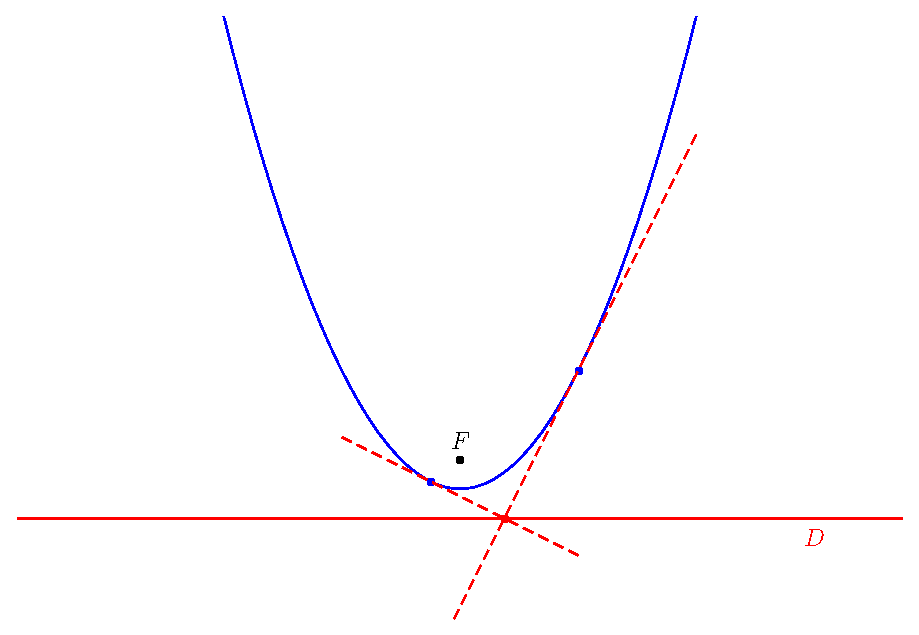
\includegraphics{../images/AGbd-1}$$
}
}
